\documentclass[a0paper]{tikzposter}

\usepackage{mathptmx}
\usepackage{array}
\usepackage{multicol}
\usepackage{tabularx}


\definebackgroundstyle{dlsbackground}{
    \node [anchor=south west, inner sep=0, line width=0] at (bottomleft)
        {
\includegraphics{diamond-background.png}};
    \node [anchor=south east, inner sep=0, line width=0,
           xshift=-1.25cm, yshift=1.16cm]
        at (bottomleft -| topright)
        {
\includegraphics[scale=1.52]{diamond_logo.eps}};
}

\title{\begin{minipage}{\linewidth}\centering
    A New Transverse and Longitudinal Bunch by Bunch Feedback Processor
    \vspace{1cm}
\end{minipage}
}

\author{M.G.~Abbott, G.~Rehm, I.S.~Uzun\textsuperscript{1}}
\institute{
    Diamond Light Source, Oxfordshire, UK \\
    \textsuperscript{1}STFC, UK
}

\hyphenpenalty=4000
\setlength{\columnsep}{2cm}

\usetheme{Envelope}
\usebackgroundstyle{dlsbackground}


% TikZ settings for text
\colorlet{normal colour}{green!60!blue!20}  % Normal coloured filled areas
\colorlet{accent colour}{orange!25}         % Accented filled areas
\tikzset{
    highlight fill/.style={fill=normal colour},
    small box/.style={
        draw, rectangle, thick, highlight fill},
    inline text/.style={
        baseline=(current bounding box.base),
        every node/.append style={anchor=base, font=\small},},
    mul/.style={
        draw=black, circle, thick, highlight fill, inner sep=0.5ex},
}

% Useful for inline boxes
\newcommand\smallbox[2][small box]{\tikz [inline text] \node [#1] {#2};}


\begin{document}

\maketitle



\begin{columns}
\column{0.3}

\block{Abstract and Context}{
\textbf{Abstract}\quad
We describe the development of firmware to support Longitudinal Bunch by Bunch
Feedback at Diamond Light source.  As well as feedback, the system supports
complex experiments and the capture of detailed electron beam diagnostics.  In
this paper we describe the firmware development and some details of the
processing chain.  We focus on some of the challenges of FPGA development from
the perspective of a software engineer.

\vskip1cm

We are transitioning from Libera Bunch-by-Bunch platform (based on 15 year old
Virtex-II Pro FPGA) to MicroTCA, which provides access to more up to date
hardware.
}


\column{0.7}
\block{New Hardware Platform}{
\begin{multicols}{2}

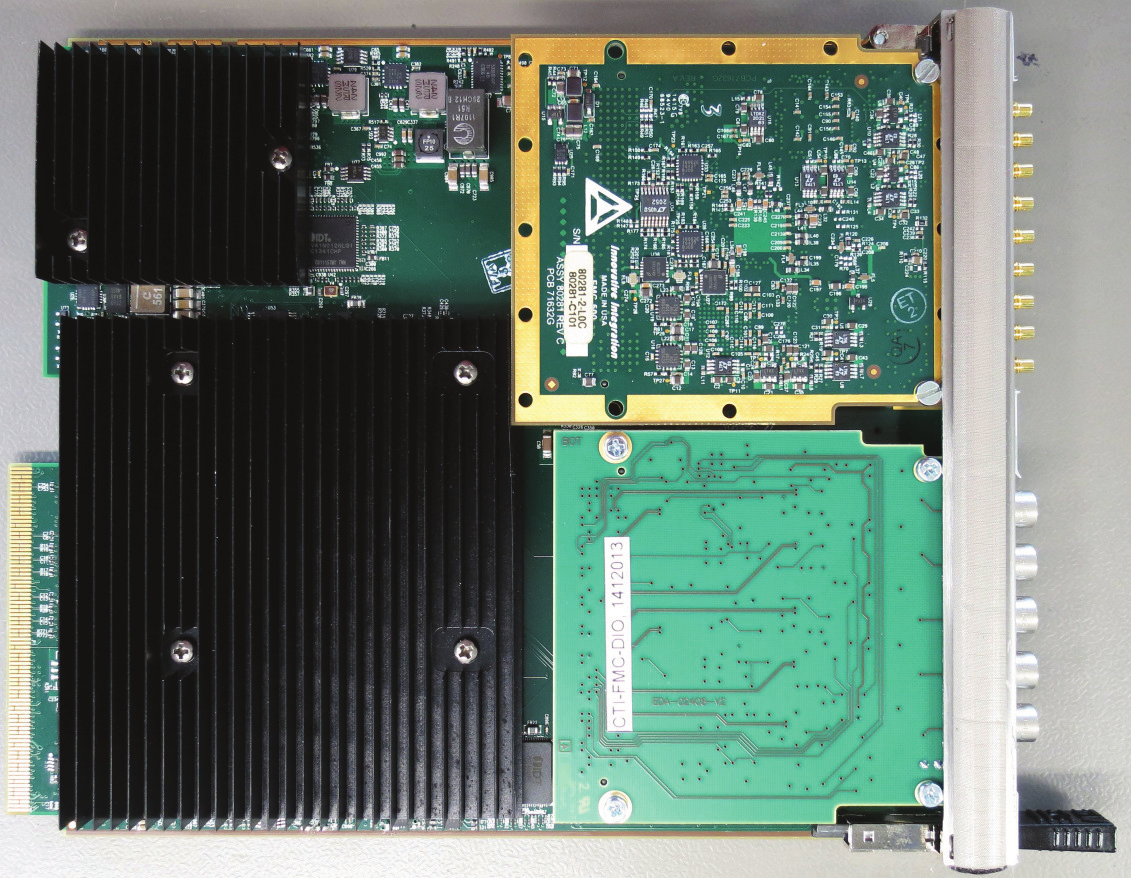
\includegraphics[width=\linewidth]{THPHA115f1.png}

Here we see the chosen hardware platform, with a 500\,MSPS ADC/DAC FMC card at
top right, and a Virtex-7 690 FPGA under the heatsink at bottom left.

\medskip

\begin{description}
\item[FMC-500M]
    High Pin Count FMC providing dual channel 500\,MS/s 14-bit ADC and dual
    channel 1230\,MS/s 16-bit DAC.  This will support bunch-by-bunch operation
    at our machine RF frequency of 500\,MHz.
\item[AMC525]
    Double width AMC card with two HPC FMC slots, 2\,GB of fast on board DRAM
    and 128\,MB of slower DRAM connected to a Virtex-7 690 FPGA, supporting an 8
    lane gen3 PCIe connection over the MicroTCA backplane.  This is where all
    the FPGA firmware will run, and the fast backplane connection will allow us
    to do a lot of data processing in the associated CPU.
\end{description}

\end{multicols}
}

\end{columns}


\block{Data Processing Paths through Bunch-by-Bunch Processor}{
\begin{tabular}{m{0.45\linewidth}m{0.50\linewidth}}
\includegraphics[width=\linewidth]{figures-1.pdf}
&
\begin{minipage}{\linewidth}
    This figure shows the data processing for a single LMBF/TMBF channel:

    \medskip

    \begin{tabularx}{\linewidth}{cX}
    \smallbox{OVF} &
        ADC input overflow detection (programmable threshold) \\
    \smallbox{FIR} &
        I/O compensation filter (8 tap FIR) \\
    \smallbox{MMS} &
        bunch position and motion measurement, measures min/max/sum
        and sum of squares \\
    \smallbox{$\div$N} &
        bunch by bunch decimation (average over programmable count) \\
    \smallbox{BB FIR} &
        bunch by bunch filter (8 tap FIR per bunch) \\
    \smallbox{$\times$N} &
        bunch by bunch interpolation \\
    \smallbox{G} &
        gain control (scale by power of 2) \\
    \smallbox{DLY} &
        output alignment delay \\
    \smallbox[mul, inner sep=2pt]{$\sim$} &
        controllable oscillator (NCO) \\
    \end{tabularx}

    \bigskip

    Overflow detection and saturation is implemented at each point where
    overflow can occur.
\end{minipage}
\end{tabular}
}


\block{Overview of Implementation}{
\begin{tikzpicture}
    \path
        node (top) {
            \includegraphics[width=0.45\linewidth]{figures-4.pdf}}
        (top.north east) ++(1cm,0) node [anchor=north west] (flows) {
            \includegraphics[width=0.2\linewidth]{figures-2.pdf}}
        (flows.north east) node [anchor=north west] (interconnect) {
            \includegraphics[width=0.25\linewidth]{figures-3.pdf}}
        (interconnect.south-|top.east) node [anchor=north west] (dsp top) {
            \includegraphics[width=0.5\linewidth]{figures-5.pdf}}
    ;

\path (top.south) node [anchor=north] {\begin{minipage}{0.45\linewidth}
\textbf{Overview of top level FPGA design.}

The ``interconnect'' at the top connects to all of the hardware resources
provided by the AMC525 carrier card, including 8-lane PCIe and 2\,GB of fast
DRAM.  The rest of the this figure shows connections to the FMC cards, clocking
and control, and the data processing core ``dsp main''.
\end{minipage}};


\path (dsp top.south) node [anchor=north] {\begin{minipage}{0.45\linewidth}
\textbf{Overview of data processing implementation for a single channel.}

The symbol \smallbox[small box, fill=accent colour]{ADC} represents points were
data is interchanged with the other channel depending on whether TMBF or LMBF
mode has been selected.

\end{minipage}};

\end{tikzpicture}

}



\end{document}
